\FloatBarrier
\subsection{Pattern architetturale MVP}

Un' importante fase durante la progettazione di applicazioni software \`e la scelta di un'opportuna architettura, che definisce le linee guida allo sviluppo del progetto. Definire bene tale processo \`e utile sia per standardizzare il modello di sviluppo del progetto corrente, sia per le applicazioni
future.
L'impiego di un adeguato pattern porta numerosi vantaggi tra cui:
\begin{itemize}
\item Incrementa il riutilizzo del codice.
\item Facilita il lavoro in team e la pianificazione del progetto, dividendo
quest'ultimo in componenti indipendenti delegabili a gruppi di lavoro
differenti.
\item Aiuta la manutenzione del codice.
\item Aumenta la flessibilit\`a delle applicazioni e incrementa della scalabilit\`a.
\end{itemize}
Il Model-View-Presenter (MVP) \`e un pattern architetturale usato principalmente quando si vogliono creare User Interfaces. 
Il pattern MVP Separa la parte di gestione dei dati di un'applicazione dalla loro visualizzazione e manipolazione attraverso l'interfaccia utente. 
\begin{figure}[htbp]
\centering%
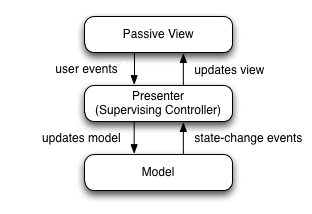
\includegraphics[scale=0.7]{MVP.png}%
\caption{Diagramma del Model-View-Presenter MVP}\label{fig:mvp}%
\end{figure}\\
Questo pattern \`e composto da tre elementi:
\begin{description}
\item[Model] \`e un'interfaccia che definisce i dati da visualizzare ed incapsula lo stato dell'applicazione.
\item[View] \`e un'interfaccia responsabile della visualizzazione dei
dati e delle informazioni, raccoglie gli input dell'utente e mai la manipolazione dei dati avviene in maniera diretta ma sempre attraverso un'interfaccia. Questo tipo di approccio consente di gestire facilmente eventuali modifiche alla GUI (Graphical User Interface) che non richiederanno mai l'aggiornamento del presenter.
\item[Presenter]  \`e colui che, oltre ad aggiornare la vista, interagisce con il model,che pu\`o essere identificato sia come lo stato di un oggetto che come dati persistenti in un'applicazione, in base alle richieste ricevute dalla view.
\end{description}
Nelle viste vi \`e una relazione uno a uno con i presenters e ci\`o permette a questi di osservare le loro viste e reagire agli eventi. Siccome le viste non possono interagire direttamente con altre viste, i presenters devono scambiare i dati con gli altri presenters. Per ottenere tale comunicazione  fra presenters, si fa uso dell' Event Bus, un oggetto in grado di trasmettere e filtrare le notifiche(figura \ref{fig:mvpEB}).

\FloatBarrier
\begin{figure}[!htb]
\centering%
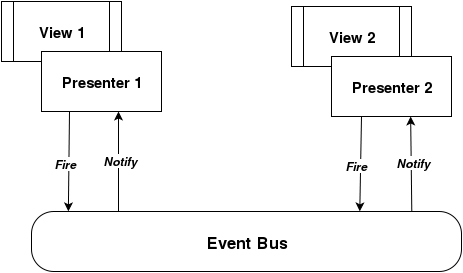
\includegraphics[scale=0.5]{EBdiagram.png}%
\caption{Comunicazione tra unit\`a del software che non sono direttamente collegate tra loro. Ognuna di esse pu\`o inviare eventi all'Event Bus ed essere in "ascolto" di  particolari eventi.}\label{fig:mvpEB}%
\end{figure}

\FloatBarrier
\begin{figure}[!htb]
\centering
\includegraphics[scale=0.45,angle=270]{GWTappMVP.png}
\caption{Implementazione client seguendo pattern MVP}
\label{fig:mvpApp}
\end{figure}

